%!TEX program = pdflatex
% ============================================================
%  Presentación ELA-NOM — Sustentación de Maestría
%  Juan Sotelo Aguilar · Universidad de La Sabana · 2026
% ============================================================
\documentclass[aspectratio=169, 9pt]{beamer}

\usepackage[T1]{fontenc}
\usepackage[utf8]{inputenc}
\usepackage[spanish,es-nodecimaldot]{babel}
\usepackage{lmodern}
\usepackage{microtype}
\usepackage{amsmath, amssymb, bm}
\usepackage{booktabs}
\usepackage{array}
\usepackage{colortbl}
\usepackage{multirow}
\usepackage{graphicx}
\usepackage{tikz}
\usetikzlibrary{positioning}
\usepackage{xcolor}
\usepackage{hyperref}

% Ayuda a LaTeX a romper líneas largas en columnas estrechas de Beamer
\setlength{\emergencystretch}{2.5em}
\tolerance=9999

\usetheme{ELANOM}

% ── Metadatos ──────────────────────────────────────────────────────────────────
\title{ELA-NOM}
\subtitle{Diseño e implementación del modelo ELA-NOM:\\
          un \textit{nowcasting} elección-agnóstico para la intención de voto\\
          aplicado a elecciones locales en Colombia 2023}
\author{Juan Sotelo Aguilar}
\institute{Maestría en Analítica Aplicada · Universidad de La Sabana}
\date{Agosto 2026}

% ── Columnas de tabla con ancho fijo ──────────────────────────────────────────
\newcolumntype{L}[1]{>{\raggedright\arraybackslash}p{#1}}
\newcolumntype{C}[1]{>{\centering\arraybackslash}p{#1}}
\newcolumntype{R}[1]{>{\raggedleft\arraybackslash}p{#1}}

\begin{document}

% sections/00_portada.tex
\newcommand{\portada}{%

% ── PORTADA ─────────────────────────────────────────────────
\begin{frame}[plain]
\begin{tikzpicture}[remember picture, overlay]
  % Fondo
  \fill[elanBG] (current page.north west) rectangle (current page.south east);
  % Banda dorada superior
  \fill[elanGold] ([yshift=-0.5cm]current page.north west)
                  rectangle ([yshift=-0.56cm]current page.north east);
  % Logo Sabana arriba a la derecha
  \node[anchor=north east, xshift=-0.5cm, yshift=-0.6cm] at (current page.north east)
    {
\includegraphics[height=1cm]{img/logos/unisabana-logo.png}};
  % Título
  \node[anchor=center, yshift=1.4cm, text width=14cm, align=center] at (current page.center)
    {{\color{elanGold}\fontsize{22}{26}\selectfont\bfseries ELA-NOM}\\[0.3em]
     {\color{elanWhite}\fontsize{14}{18}\selectfont\itshape Election-Agnostic Nowcasting Model}};
  % Subtítulo
  \node[anchor=center, yshift=0.1cm, text width=14cm, align=center] at (current page.center)
    {{\color{elanGray}\normalsize Un modelo de predicción electoral sin encuestas\\para el entorno local latinoamericano}};
  % Separador
  \fill[elanPanel] ([yshift=-1.5cm]current page.center)
                   rectangle +(\paperwidth, 0.04);
  % Autor e institución
  \node[anchor=center, yshift=-2.1cm, text width=14cm, align=center] at (current page.center)
    {{\color{elanWhite}\small\textbf{Juan Soage}}\\[0.15em]
     {\color{elanGray}\footnotesize Universidad de La Sabana · Maestría en Analítica e Inteligencia de Negocios}\\[0.15em]
     {\color{elanGray}\footnotesize Junio 2026}};
  % Banda dorada inferior
  \fill[elanGold] ([yshift=0.5cm]current page.south west)
                  rectangle ([yshift=0.56cm]current page.south east);
\end{tikzpicture}
\end{frame}

% ── AGENDA ──────────────────────────────────────────────────
\begin{frame}{Agenda}
\begin{columns}[T]
\column{0.5\textwidth}
  \begin{enumerate}\itemsep0.5em
    \item \highlight{Motivación} y gap empírico
    \item \highlight{Pregunta} e hipótesis
    \item \highlight{Etapa 1 — Bolivia}\\
          {\small SOMEN-DC: límites del estado del arte}
    \item \highlight{Etapa 2 — Costa Rica}\\
          {\small Reconstrucción temporal Weibull}
  \end{enumerate}
\column{0.5\textwidth}
  \begin{enumerate}\setcounter{enumi}{4}\itemsep0.5em
    \item \highlight{Etapa 3 — Colombia}\\
          {\small Dataset, modelado, ElasticNet}
    \item \highlight{Resultados} Colombia 2023
    \item \highlight{Validación prospectiva} 2026
    \item \highlight{Conclusiones} y trabajo futuro
  \end{enumerate}
\end{columns}
\vspace{0.8em}
\begin{tikzpicture}
  \fill[elanPanel] (0,0) rectangle (\textwidth, 0.7);
  \node[anchor=west, xshift=0.3cm, yshift=0.35cm] at (0,0)
    {{\color{elanGold}\small\bfseries Duración:}
     {\color{elanGray}\small\ 30 min presentación + preguntas del jurado}};
\end{tikzpicture}
\end{frame}

}% fin \portada

% DIAPOSITIVA 3: El problema
\begin{frame}{El problema: saber quién va a ganar es costoso}
  \begin{columns}[T]
    \begin{column}{0.52\textwidth}
      \textbf{La industria de pronósticos electorales}
      \begin{itemize}
        \item Industria global de opinión pública:\\
              \num{\$153 mil millones} facturados en 2024
        \item Colombia: más de \num{\$700 mil millones COP} (2024)
        \item Plataformas predictivas alternativas:\\
              Polymarket mueve más de \num{1 billón USD} en contratos de predicción
      \end{itemize}
      \vspace{0.5em}
      \textbf{Tres retos del sector en Colombia}
      \begin{itemize}
        \item \alrt{Regulatorio:} Ley 2494/2025 endureció divulgación.
              \textbf{GAD3} se retiró del país en 2026
        \item \alrt{Cobertura:} más de \num{1.100 municipios}; encuestadoras
              cubren solo 10-12 ciudades
        \item \alrt{Costo:} una encuesta multimuestra es inviable
              para elecciones subnacionales
      \end{itemize}
    \end{column}
    \begin{column}{0.44\textwidth}
      \vspace{0.3em}
      \begin{block}{La pregunta natural}
        ¿La actividad ciudadana en redes sociales dice algo sobre cómo va a votar el colombiano?
      \end{block}
      \vspace{0.5em}
      \begin{block}{Definición: \textit{Nowcasting}}
        Estimación del valor \textbf{actual} de una variable subyacente difícil de observar directamente, a partir de señales disponibles en tiempo real.
      \end{block}
    \end{column}
  \end{columns}
\end{frame}

% DIAPOSITIVA 4: Literatura
\begin{frame}{De los modelos econométricos a las redes sociales}
  \begin{itemize}
    \item \textbf{1970s-2000s:} primeros modelos de nowcasting electoral con variables
          económicas y de aprobación (VAR, ARCH/GARCH): alta precisión histórica
    \item \textbf{2016:} golpe de gracia. Ningún modelo predijo \textbf{Trump} ni el \textbf{Brexit}
    \item \textbf{2009:} Tumasjan \textit{et al.}: menciones en Twitter como estimador insesgado
          de participación electoral; MAE inferior al 2\% con millones de tweets
    \item \textbf{2010s-2020s:} modelos híbridos (redes más variables económicas) mejoran resultados
          pero requieren infraestructura de extracción masiva, inviable fuera de academia
    \item \textbf{Brito \& Andeato (2020s):} \kw{SOMEN-DC}: \textit{Social Media Electoral Nowcasting
          During Campaign}. Promete superar encuestadoras con interacciones de candidatos
  \end{itemize}

  \vspace{0.4em}
  \begin{alertblock}{Problema identificado en SOMEN-DC}
    Tres limitaciones estructurales que los autores no resuelven:
    \begin{itemize}
      \item \alrt{Techo encuestocéntrico:} la variable objetivo \textbf{son las encuestas}, no los resultados
      \item \alrt{During-Campaign:} requiere scraping diario desde el primer día de campaña
      \item \alrt{No transferibilidad:} pesos específicos a cada elección; imposible generalizar
    \end{itemize}
  \end{alertblock}
\end{frame}

% DIAPOSITIVA 5: Pregunta central
\begin{frame}{Pregunta de investigación}
  \begin{block}{Pregunta central}
    ¿Es posible diseñar un modelo de \textit{nowcasting} electoral \textbf{elección-agnóstico},
    cuyos parámetros se entrenen con múltiples contiendas pasadas y sean
    \textbf{transferibles} a elecciones nuevas, que opere \textbf{sin encuestas},
    usando exclusivamente señales de redes sociales?
  \end{block}

  \vspace{0.25em}
  \begin{columns}[T]
    \begin{column}{0.48\textwidth}
      {\small\textbf{\color{barBlue}Preguntas derivadas (P)}}
      \begin{itemize}\small
        \item[\textbf{P1}] ¿Tienen las interacciones digitales poder predictivo real sobre el comportamiento electoral en Colombia?
        \item[\textbf{P2}] ¿Es posible reconstruir matemáticamente el historial de interacciones sin haber recolectado datos en tiempo real?
        \item[\textbf{P3}] ¿Qué métrica digital es el predictor más informativo y robusto?
        \item[\textbf{P4}] ¿Cuántas contiendas de entrenamiento son necesarias para que el modelo alcance desempeño estable?
      \end{itemize}
    \end{column}
    \begin{column}{0.48\textwidth}
      {\small\textbf{\color{barBlue}Preguntas metodológicas (PM)}}
      \begin{itemize}\small
        \item[\textbf{PM1}] ¿Es posible replicar el SOMEN-DC en una elección no tratada por sus autores?
        \item[\textbf{PM2}] ¿Se confirman empíricamente las tres limitaciones estructurales del SOMEN-DC?
        \item[\textbf{PM3}] ¿Es posible reconstruir el historial de interacciones con precisión suficiente para construir un dataset de entrenamiento retroactivo?
        \item[\textbf{PM4}] ¿Es el modelo transferible a un formato electoral diferente al de entrenamiento?
      \end{itemize}
    \end{column}
  \end{columns}
\end{frame}

% DIAPOSITIVA 6: Diseño general
\begin{frame}{Diseño empírico: tres etapas}
  \begin{columns}[T]
    \begin{column}{0.42\textwidth}
      \vspace{0.3em}
      \begin{center}
      \begin{tikzpicture}[node distance=0.5cm]
        \tikzstyle{box}=[rectangle, rounded corners=3pt, draw=barBlue,
                         fill=tableBand, minimum width=3.8cm, minimum height=0.7cm,
                         text width=3.6cm, align=center, font=\small\bfseries]
        \tikzstyle{lbl}=[font=\scriptsize, text=subtleGray, align=center,
                         text width=3.6cm]
        \tikzstyle{arr}=[->, thick, color=barBlue]

        \node[box] (bol) {Etapa 1: Bolivia};
        \node[lbl, below=0.15cm of bol] (lbol) {Replicación SOMEN-DC\\PM1, PM2};
        \node[box, below=0.4cm of lbol] (cr) {Etapa 2: Costa Rica};
        \node[lbl, below=0.15cm of cr] (lcr) {Restaurador Weibull\\P2, PM3};
        \node[box, below=0.4cm of lcr] (col) {Etapa 3: Colombia};
        \node[lbl, below=0.15cm of col] (lcol) {Modelo ELA-NOM\\P1, P3, P4};
        \node[box, below=0.4cm of lcol] (val) {Validación 2026};
        \node[lbl, below=0.15cm of val] (lval) {Transferibilidad\\PM4};

        \draw[arr] (bol) -- (cr);
        \draw[arr] (cr) -- (col);
        \draw[arr] (col) -- (val);
      \end{tikzpicture}
      \end{center}
    \end{column}
    \begin{column}{0.54\textwidth}
      \textbf{Variable objetivo:}
      \[
        \hat{y}_c = f\!\left(\mathbf{x}_c\right) \in (0,1)
        \quad\text{con}\quad
        \sum_{j \in \mathcal{C}_e} \hat{y}_{c_j} = 1
      \]
      \small
      $f\!: \mathbb{R}^d \to (0,1)$, escalar por candidato.
      La restricción de suma se aplica por normalización posterior.

      \vspace{0.5em}
      \textbf{Supuesto central:}
      \begin{itemize}
        \item Los parámetros de $f$ se aprenden con \textbf{múltiples} elecciones pasadas $\mathcal{E}$
        \item Se aplican \textbf{sin reentrenamiento} a elecciones nuevas
        \item Variable objetivo: \kw{cuota electoral observada} (no intención de voto latente)
      \end{itemize}
    \end{column}
  \end{columns}
\end{frame}

% DIAPOSITIVA 7: Bolivia -- diseño
\begin{frame}{Etapa 1: Bolivia -- replicación del SOMEN-DC}
  \textbf{Elección seleccionada}
  \begin{itemize}
    \item Bolivia, 2.ª vuelta presidencial, 19 oct.\ 2025
    \item Rodrigo Paz Pereira vs.\ Jorge ``Tuto'' Quiroga
    \item Elección bipolar, no tratada previamente por SOMEN-DC
  \end{itemize}
  \vspace{0.4em}
  \textbf{Dataset}
  \begin{itemize}
    \item \num{153} días de campaña (18 may.\ al 18 oct.\ 2025)
    \item Plataformas: Facebook, Instagram, TikTok, Twitter/X
    \item \num{308} observaciones, \num{26} características
    \item Variable objetivo: interpolación de \num{14} encuestas
          anclada al resultado real: Paz \num{54,53\%}, Quiroga \num{45,47\%}
  \end{itemize}
  \vspace{0.4em}
  \textbf{Modelos entrenados:} 6 especificaciones
  (lineal, lineal más PCA, MLP-BP, MLP-BP más PCA, GRNN)
\end{frame}

% DIAPOSITIVA 8: Bolivia -- gráfica serie de tiempo
\makered
\begin{frame}{Etapa 1: Bolivia -- evolución de la predicción}
  \begin{center}
    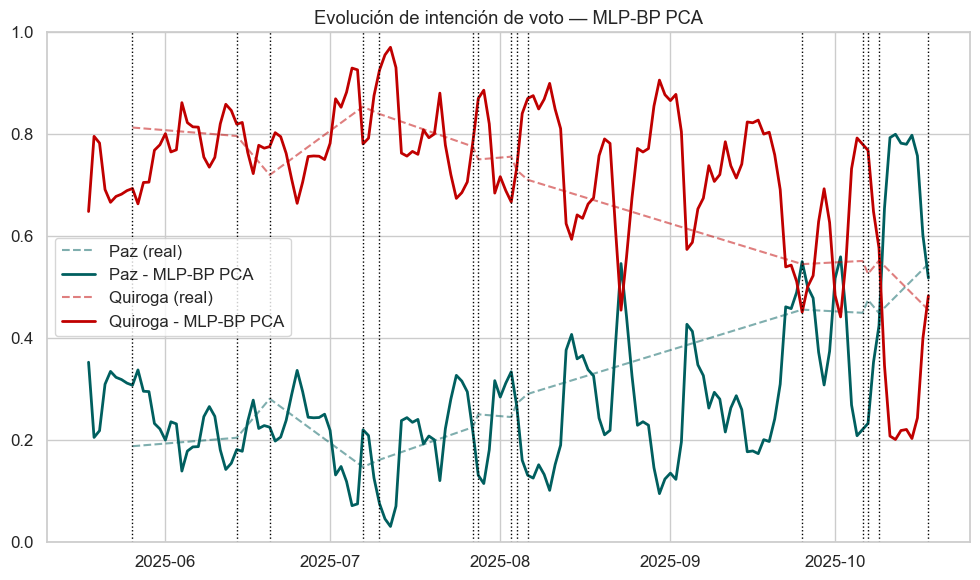
\includegraphics[width=0.88\textwidth]{img/mlp_bp_pca_timeseries.png}
  \end{center}
  {\footnotesize\color{subtleGray}\centering
    Evolución predicha vs.\ encuestas -- MLP-BP+PCA (modelo ganador)}
\end{frame}
\makeblue

% DIAPOSITIVA 9: Bolivia -- resultados
\begin{frame}{Etapa 1: Bolivia -- resultados (día de la elección)}
  \vspace{-0.1em}
  \begin{center}
  \small
  \rowcolors{2}{tableBand}{white}
  \begin{tabular}{L{4.2cm} C{2.0cm} C{1.6cm} C{1.6cm}}
    \toprule
    \rowcolor{barBlue}
    {\color{white}\textbf{Modelo}} &
    {\color{white}\textbf{Pred.\ Paz}} &
    {\color{white}\textbf{MAE}} &
    {\color{white}\textbf{MAPE}} \\
    \midrule
    Baseline (última encuesta) & 36,50\% & 0,1803 & 33,1\% \\
    Regresión lineal           & 24,85\% & 0,2968 & 54,4\% \\
    Regresión lineal + PCA     & 23,38\% & 0,3115 & 57,1\% \\
    MLP-BP                     & 46,91\% & 0,0762 & 14,0\% \\
    \rowcolor{tableBand}
    \textbf{MLP-BP + PCA}      & \textbf{51,74\%} & \textbf{0,0279} & \textbf{5,1\%} \\
    GRNN                       & 34,67\% & 0,1986 & 36,4\% \\
    \midrule
    Resultado real             & \num{54,53\%} & {-} & {-} \\
    \bottomrule
  \end{tabular}
  \end{center}

  \vspace{0.2em}
  \begin{columns}[T]
    \begin{column}{0.55\textwidth}
      \small
      \textbf{Observación metodológica:} MAE y RMSE son idénticos porque $n=1$
      (un solo punto de evaluación). Se reporta MAE y MAPE; la tabla eliminó
      la columna RMSE redundante. [\corr{Corrección 1.9}]
    \end{column}
    \begin{column}{0.41\textwidth}
      \begin{block}{\textbf{PM1}: Respondida}
        \small La replicación es posible.\\
        MLP-BP+PCA supera 6 veces al baseline.
      \end{block}
    \end{column}
  \end{columns}
\end{frame}

% DIAPOSITIVA 10: Bolivia -- limitaciones, PM2
\begin{frame}{Etapa 1: Bolivia -- confirmación de las tres limitaciones}
  \begin{columns}[T]
    \begin{column}{0.52\textwidth}
      \textbf{Las tres limitaciones se verificaron empíricamente:}
      \begin{itemize}
        \item \alrt{No transferibilidad confirmada:}\\
              Los pesos del MLP-BP son específicos de Bolivia.\\
              No existe mecanismo para exportarlos a Colombia.
        \vspace{0.3em}
        \item \alrt{Rezago estructural:}\\
              En la última semana Paz remontó en encuestas.\\
              El modelo, con interacciones acumuladas, no lo capturó.
        \vspace{0.3em}
        \item \alrt{Disociación TikTok:}\\
              Picos de TikTok inyectaban varianza espuria\\
              cuando la intención de voto estaba estacionaria.
      \end{itemize}
    \end{column}
    \begin{column}{0.44\textwidth}
      \begin{alertblock}{\textbf{PM2}: Respondida}
        El paradigma \textit{During-Campaign} no escala:\\
        requiere infraestructura desde el día 1 y\\
        produce pesos no exportables.\\[0.4em]
        \textbf{Conclusión:} necesitamos un enfoque\\
        \textit{fuera de campaña} y agnóstico a la elección.
      \end{alertblock}
      \vspace{0.4em}
      \small
      \textbf{Siguiente paso:} resolver el problema del histórico.
      ¿Cómo conocer el estado de las interacciones en el pasado sin
      haber recolectado datos en tiempo real?
    \end{column}
  \end{columns}
\end{frame}

% DIAPOSITIVA 10: El problema del histórico
\begin{frame}{Etapa 2: Costa Rica -- el problema del histórico}
  \begin{columns}[T]
    \begin{column}{0.54\textwidth}
      \textbf{Obstáculo técnico central:}
      \begin{itemize}
        \item Las plataformas solo muestran el \textbf{total acumulado hoy}
        \item Una publicación de oct.\ 2023 tiene hoy los likes de ago.\ 2026
        \item El tráfico póstumo (post-elección) \textbf{contamina} cualquier
              extracción retrospectiva estática
      \end{itemize}
      \vspace{0.3em}
      \textbf{Solución propuesta:}\\
      Modelar la función de crecimiento acumulado $F(t)$ de cada plataforma.
      Si conocemos la forma de la curva, podemos estimar cuántas interacciones
      tenía cualquier publicación en cualquier momento pasado.

      \vspace{0.3em}
      \textbf{Panel de calibración:} 1.ª vuelta Costa Rica, 1 feb.\ 2026
      \begin{itemize}
        \item 30 días de observación (15 antes, 15 después)
        \item 4 candidatos, 4 plataformas
        \item \num{1.922} publicaciones, \num{19.439} pares $(t, F)$
      \end{itemize}
    \end{column}
    \begin{column}{0.42\textwidth}
      \begin{block}{Intuición}
        Las reacciones llegan masivamente en las primeras horas y luego decaen.
        La curva es asimétrica: arranque explosivo, caída rápida, estabilización.
      \end{block}
      \vspace{0.5em}
      \textbf{Tres familias comparadas:}
      \begin{itemize}
        \item Exponencial simple
        \item Logística (inflexión simétrica)
        \item \kw{Weibull con offset}, ganadora
      \end{itemize}
    \end{column}
  \end{columns}
\end{frame}

% DIAPOSITIVA 11: Familia Weibull -- comparación
\begin{frame}{Etapa 2: Selección de la función de crecimiento}
  \begin{center}
  {\setlength{\tabcolsep}{3pt}
  \scriptsize
  \rowcolors{2}{tableBand}{white}
  \begin{tabular}{L{2.6cm} L{3.8cm} C{1.3cm} L{4.6cm}}
    \toprule
    \rowcolor{barBlue}
    {\color{white}\textbf{Modelo}} &
    {\color{white}\textbf{Ecuación}} &
    {\color{white}\textbf{$\bar{R}^2$}} &
    {\color{white}\textbf{Diagnóstico}} \\
    \midrule
    Exponencial simple &
      $F(t) = 1 - e^{-kt}$ &
      0,182 &
      Rígido; $\alpha \equiv 1$; subestima acumulación inicial \\
    Logístico &
      $F(t) = \dfrac{1}{1+e^{-k(t-t_0)}}$ &
      0,245 &
      Inflexión simétrica forzada; inadecuado para asimetría real \\
    \rowcolor{tableBand}
    \textbf{Weibull con offset} &
      $\bm{F(t) = 1 - e^{-k(t+t_0)^{\alpha}}}$ &
      \textbf{0,449} &
      Geometría flexible ($\alpha$); adelanto inicial ($t_0$); acotada en $[0,1]$ \\
    \bottomrule
  \end{tabular}}
  \end{center}

  \vspace{0.2em}
  \begin{columns}[T]
    \begin{column}{0.55\textwidth}
      \small\textbf{Interpretación correcta de los parámetros} \corr{[Corr.\ 1.6]}
      \begin{itemize}\small
        \item $k$: \textbf{tasa} de acumulación (no parámetro de escala clásico)
        \item $\alpha < 1$: acumulación desacelera (Facebook, Instagram, TikTok)
        \item $\alpha > 1$: tasa de acumulación \textbf{crece} (Twitter/X: $\alpha = 1{,}14$)
        \item $t_0 > 0$: \textbf{adelanto de origen}; $F(0) > 0$; modela interacciones
              previas al primer día de observación completo
      \end{itemize}
    \end{column}
    \begin{column}{0.41\textwidth}
      \begin{exampleblock}{Nota sobre $R^2$ moderado}
        \small El \num{66,8\%} de la varianza total es intra-publicación (ruido irreducible).
        El modelo captura la \textbf{forma global} de la curva, suficiente para la
        reconstrucción histórica.
      \end{exampleblock}
    \end{column}
  \end{columns}
\end{frame}

% DIAPOSITIVA 12: Parámetros calibrados
\addtocounter{framenumber}{1}

% DIAPOSITIVA nueva: Costa Rica -- ganadora vs. resto
\begin{frame}{Etapa 2: La ganadora es indistinguible del resto}
  \begin{center}
    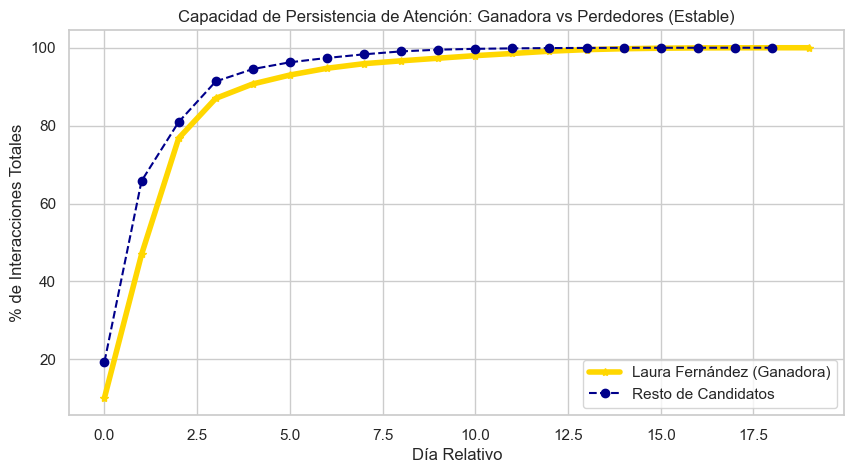
\includegraphics[width=0.80\textwidth]{img/costa_rica_ganadora.png}
  \end{center}
  {\footnotesize\color{subtleGray}\centering
    Laura Fernández (ganadora) vs.\ resto de candidatos.
    Sin diferencia estadísticamente significativa en ningún día del panel.
    El patrón de crecimiento es una propiedad de la \textbf{plataforma}, no del candidato.}
\end{frame}

% DIAPOSITIVA: Precisión proyectiva -- tabla MAPE
\addtocounter{framenumber}{1}

% DIAPOSITIVA nueva: MAPE convergencia + distribución de errores
\addtocounter{framenumber}{1}

% DIAPOSITIVA: Ajuste del restaurador por plataforma
\addtocounter{framenumber}{1}

% sections/05_etapa3_colombia.tex
\newcommand{\etapacolombia}{%

\begin{frame}{Dataset: elecciones locales Colombia 2023}
\begin{columns}[c]
\column{0.50\textwidth}
  \textbf{\color{elanGold}Construcción del dataset}
  \begin{itemize}\itemsep0.4em
    \item Universo: 33 ciudades más pobladas
    \item Excluidas: Bogotá (sesgo influencer) + Piedecuesta (sin datos digitales)
    \item Universo final: \textbf{\color{elanGold}31 ciudades competitivas}
    \item Candidatos con $>$10,000 votos: \textbf{\color{elanGold}120 candidatos}
    \item Publicaciones \'unicas: \textbf{\color{elanGold}5,776}
    \begin{itemize}
      \item[\color{elanBlue}·] Facebook: 2,511
      \item[\color{elanBlue}·] Twitter/X: 2,346
      \item[\color{elanBlue}·] TikTok: 919
    \end{itemize}
    \item Ventana de captura: \textbf{14 días} previos a los comicios
    \item Cobertura digital: \textbf{92.6\%} de candidatos con publicaciones activas
  \end{itemize}
\column{0.46\textwidth}
  \begin{tikzpicture}
    \fill[elanPanel] (0,0) rectangle (5.5,5.5);
    \node[anchor=north, yshift=-0.2cm, text=elanGold, font=\bfseries\small] at (2.75,5.5)
      {Pipeline de extracción};
    \node[anchor=north, yshift=-0.9cm, text width=5.0cm] at (2.75,5.5) {
      \small
      \begin{tabular}{ll}
        \color{elanBlue}\textbf{Facebook} & Apify scraper\\
        \color{elanBlue}\textbf{Twitter/X} & Playwright headless\\
        \color{elanBlue}\textbf{TikTok} & API privada (Apify)\\
        \color{elanRed}\textbf{Instagram} & Excluido (API restrictions)\\
      \end{tabular}
    };
    \node[anchor=south, yshift=1.0cm] at (2.75,0) {
      \begin{tikzpicture}
        \fill[elanGold!20!elanPanel] (0,0) rectangle (5.0,1.3);
        \draw[elanGold, line width=0.8pt] (0,0) rectangle (5.0,1.3);
        \node[anchor=center, text=elanGold, font=\bfseries\small] at (2.5,0.95)
          {Reconstrucci\'on Weibull};
        \node[anchor=center, text=elanGray, font=\footnotesize] at (2.5,0.40)
          {aplicada a todas las publicaciones};
      \end{tikzpicture}
    };
  \end{tikzpicture}
\end{columns}
\end{frame}

\begin{frame}{Evidencia descriptiva: dominancia digital y votos}
  \begin{center}
    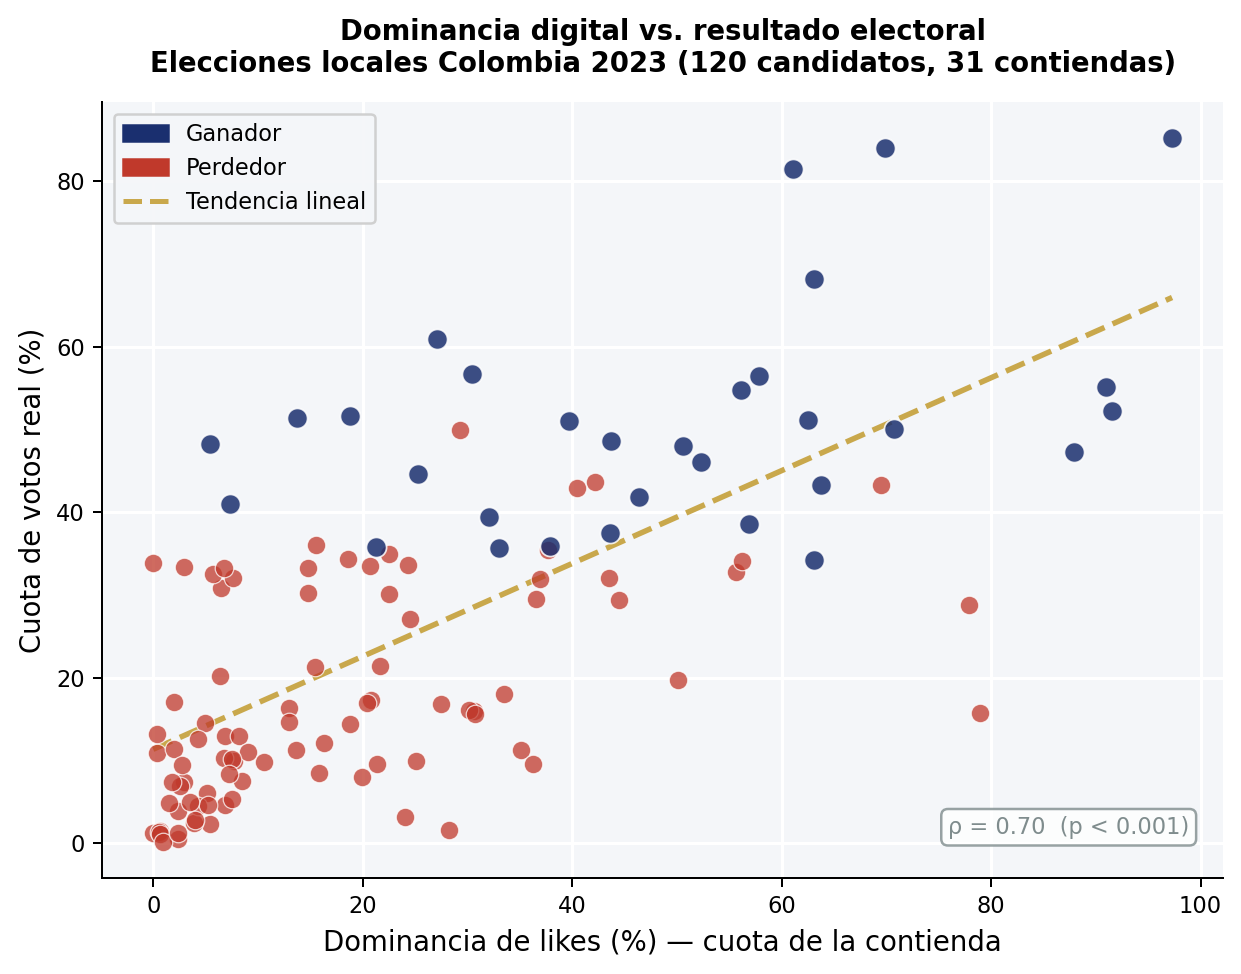
\includegraphics[width=0.78\textwidth]{img/colombia/col_scatter_dominancia_votos.png}
  \end{center}
  \vspace{-0.6em}
  \begin{tikzpicture}
    \fill[elanPanel] (0,0) rectangle (\textwidth,0.75);
    \node[anchor=west, xshift=0.3cm, yshift=0.37cm] at (0,0)
      {{\color{elanGold}\small\bfseries $\rho = 0.70$, $p < 0.001$} \quad
       {\color{elanGray}\small $\cdot$ Ganadores (azul) vs.\ perdedores (rojo) $\cdot$ 120 candidatos, 31 contiendas}};
  \end{tikzpicture}
\end{frame}

\begin{frame}{Modelado predictivo: regresión logística fraccional}
\begin{columns}[c]
\column{0.50\textwidth}
  \textbf{\color{elanGold}Especificaci\'on del modelo}\\[0.4em]
  La variable objetivo es la \textbf{cuota de voto real} $v_c \in (0,1)$.\\[0.5em]
  Dado que $v_c$ es una proporci\'on, usamos regresi\'on log\'{\i}stica fraccional (Papke \& Wooldridge, 1996):
  \[
    \mathbb{E}[v_c \mid X] = \frac{1}{1 + e^{-(\beta_0 + X^\top \beta)}}
  \]
  con predictor central:
  \[
    \text{logit}(\delta_c) = \log\!\left(\frac{\delta_c}{1-\delta_c}\right)
  \]
  \vspace{0.3em}
  \textbf{\color{elanGold}Selección de variables: ElasticNet anidado}\\
  \[
    \hat{\beta} = \arg\min_\beta \bigl\{L(\beta) + \lambda_1\|\beta\|_1 + \lambda_2\|\beta\|_2^2\bigr\}
  \]

\column{0.48\textwidth}
  \textbf{\color{elanGold}Comparativa de modelos}\\[0.2em]
  {\scriptsize M\'etricas LOCO-CV (31 contiendas)}\\[0.1em]
  {\tiny
  \begin{tabular}{@{}lrrr@{}}
    \toprule
    \color{elanWhite} Modelo & \color{elanGold} MAE & \color{elanGold} $R^2$ & \color{elanGold} T1\\
    \midrule
    Base uniforme  & 12.49 & 0.306 & 39\%\\
    Base proporcional & 12.61 & 0.185 & 71\%\\
    Reg. fraccional   & 11.52 & 0.460 & 71\%\\
    \rowcolor{elanPanel}
    \color{elanGold}\bfseries ELA-NOM & \color{elanGold}\bfseries 9.43 & \color{elanGold}\bfseries 0.518 & \color{elanGold}\bfseries 64.5\%\\
    Grad. Boosting    & 9.91 & 0.515 & 67.7\%\\
    \bottomrule
  \end{tabular}}

  \vspace{0.4em}
  \begin{tikzpicture}
    \fill[elanGold!20!elanPanel] (0,0) rectangle (5.5,1.5);
    \draw[elanGold, line width=0.7pt] (0,0) rectangle (5.5,1.5);
    \node[anchor=north, yshift=-0.1cm, text width=5.2cm] at (2.75,1.5) {
      {\color{elanGold}\bfseries\small Validaci\'on: LOCO-CV}\\
      {\color{elanGray}\footnotesize \textit{Leave-One-Contest-Out CV}: en cada pliegue
      se excluye una contienda completa y el modelo predice \textbf{fuera de muestra}.
      31~pliegues $\cdot$ unidad~=~contienda.}
    };
  \end{tikzpicture}
\end{columns}
\end{frame}

\begin{frame}{Coeficientes: estabilidad inter-pliegue (bootstrap)}
  \begin{center}
    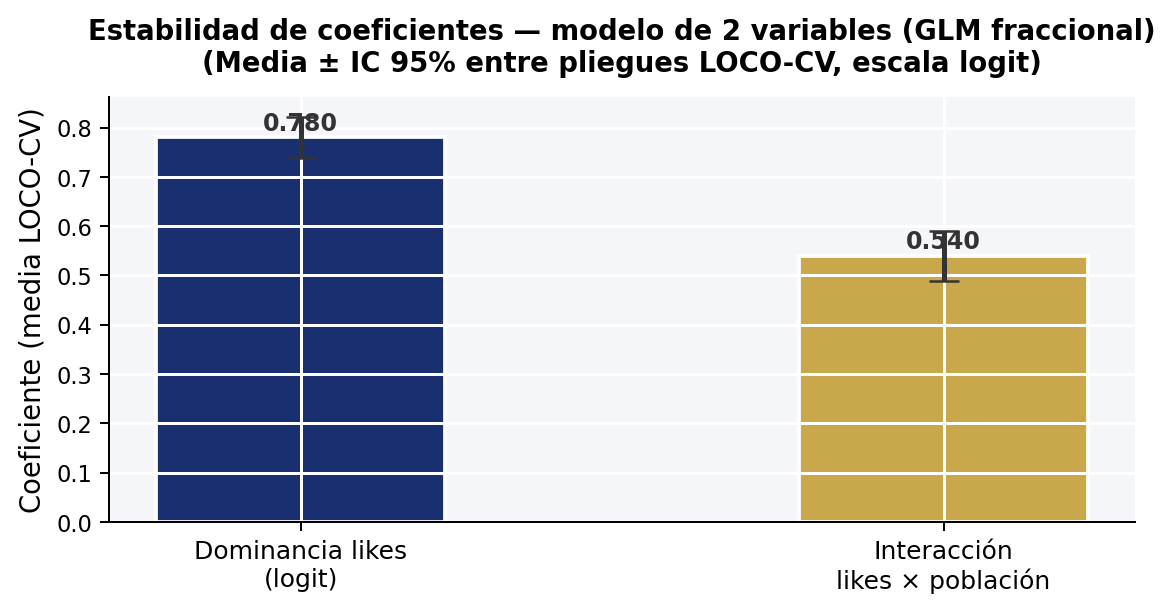
\includegraphics[width=0.82\textwidth]{img/colombia/col_coef_bootstrap.png}
  \end{center}
  \vspace{-0.4em}
  \begin{tikzpicture}
    \fill[elanPanel] (0,0) rectangle (\textwidth,0.75);
    \node[anchor=west, xshift=0.3cm, yshift=0.37cm] at (0,0)
      {{\color{elanGold}\small\bfseries Estabilidad:}
       {\color{elanGray}\small\ logit\_likes e interacción presentes en el 100\% de los pliegues de validación}};
  \end{tikzpicture}
\end{frame}

\begin{frame}{Residuales LOCO-CV: distribución del error}
  \begin{center}
    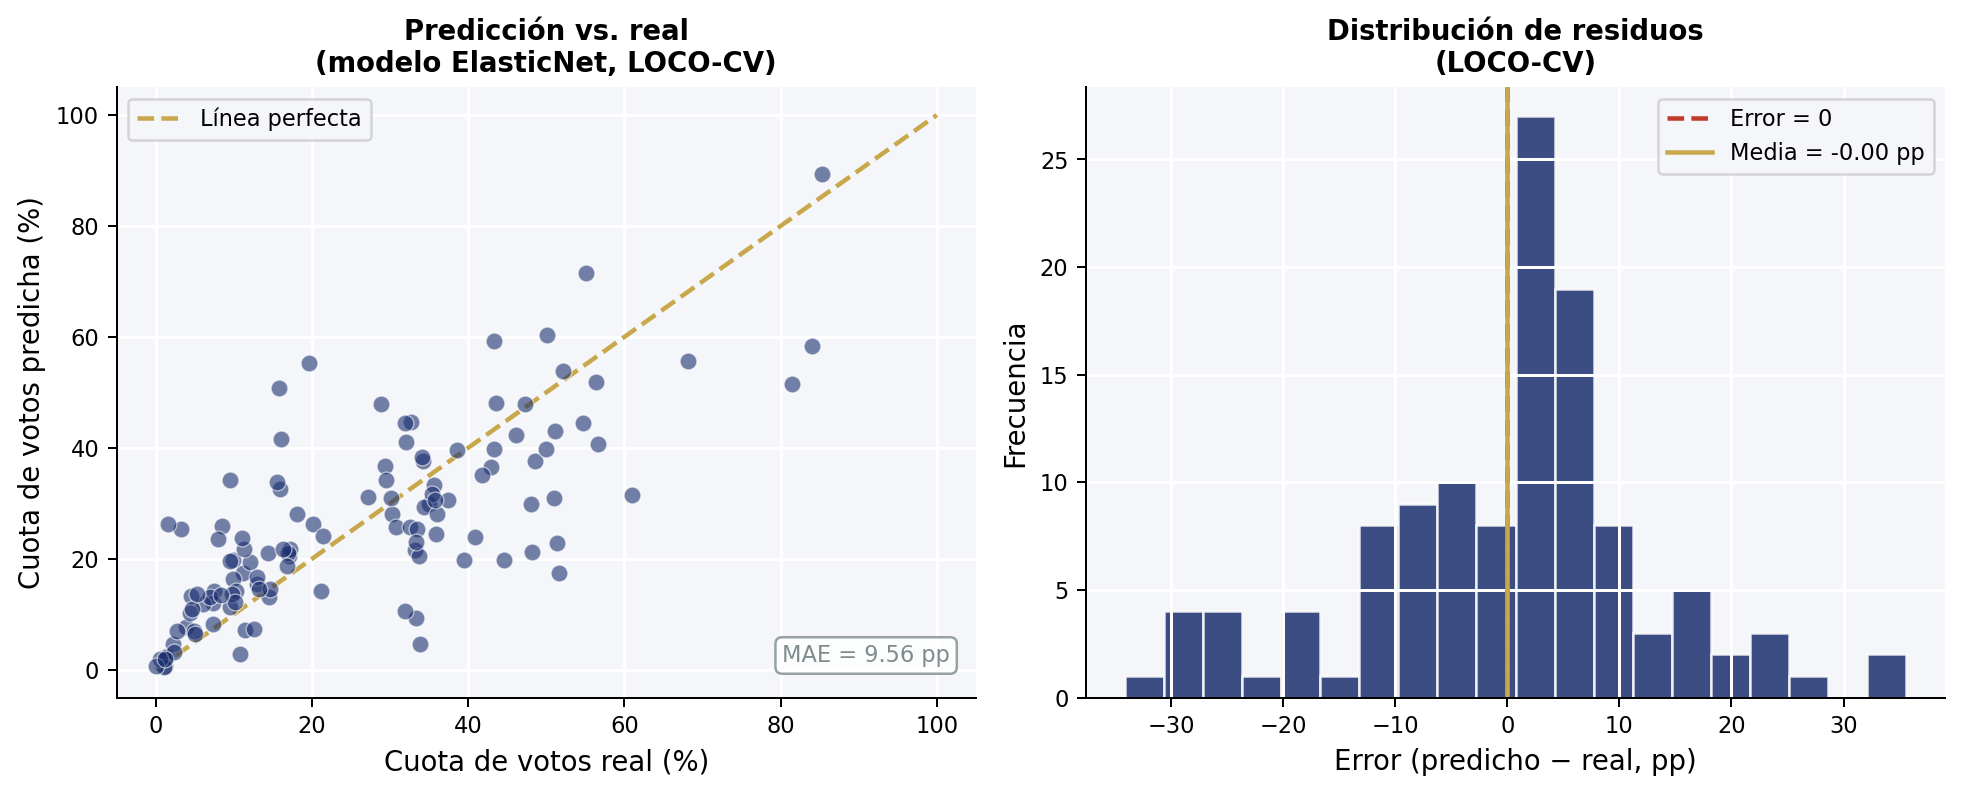
\includegraphics[width=0.85\textwidth]{img/colombia/col_loco_residuals.png}
  \end{center}
  \vspace{-0.4em}
  \begin{tikzpicture}
    \fill[elanPanel] (0,0) rectangle (\textwidth,0.75);
    \node[anchor=west, xshift=0.3cm, yshift=0.37cm] at (0,0)
      {{\color{elanGold}\small\bfseries MAE~=~9.43~pp} \quad
       {\color{elanGray}\small $\cdot$ $R^2_{\text{oos}} = 0.518$ $\cdot$ Top-1 = 64.5\% (20/31) $\cdot$ sin patrones sistem\'aticos de sesgo}};
  \end{tikzpicture}
\end{frame}

}% fin \etapacolombia

% DIAPOSITIVA 19: Pool de 9 variables y selección del modelo
\begin{frame}{Modelado: feature engineering y selección del modelo}
  \begin{columns}[T]
    \begin{column}{0.50\textwidth}
      \textbf{Pool de 9 variables} (tras filtro VIF sobre 22 candidatas)
      \begin{enumerate}\small
        \item Logit dominancia de \textit{likes}
        \item Logit dominancia de comentarios
        \item Logit dominancia de compartidos
        \item Logit \textit{likes} por publicación
        \item Logit comentarios por publicación
        \item Logit compartidos por publicación
        \item Log-población del municipio
        \item Número de candidatos en la contienda
        \item Moderador: (1) por (log-pob.\ centrada)
      \end{enumerate}
      \vspace{0.2em}
      {\small\textbf{ElasticNet} ($L_1 + L_2$): selección automática.\\
      $\hat\alpha=0{,}0475$, $\lambda=0{,}10$, StandardScaler.}
    \end{column}
    \begin{column}{0.46\textwidth}
      \textbf{Selección del modelo (AutoML)}
      \begin{itemize}\small
        \item Familias evaluadas: GLM fraccional, gradient boosting, redes neuronales,
              SVM, random forests
        \item Criterio único: MAE fuera de muestra (LOCO-CV)
        \item \kw{Ganador: GLM fraccional + ElasticNet}
      \end{itemize}
      \vspace{0.3em}
      \begin{exampleblock}{¿Por qué GLM sobre gradient boosting?}
        \scriptsize (1) Cuota $\in(0,1)$: GLM binomial+logit garantiza $\hat{y}\in(0,1)$
        (Papke \& Wooldridge, 1996). (2) Interpretabilidad: coeficientes en log-odds.
        MAE similar (9,56 vs.\  9,91 pp).
      \end{exampleblock}
    \end{column}
  \end{columns}
\end{frame}

% DIAPOSITIVA 20: LOCO-CV
\begin{frame}{Modelado: validación LOCO-CV \corr{[Corr.\ 2.3]}}
  \begin{columns}[T]
    \begin{column}{0.52\textwidth}
      \textbf{Dos fases del proceso:}
      \begin{itemize}\small
        \item \textbf{Fase 1 (evaluación):} ciclo de 31 pliegues. En cada uno se bloquea
              una ciudad completa, se hace grid search interno (120 combinaciones de
              $\hat\alpha$ y $\lambda$) sobre las 30 ciudades restantes, se elige la
              mejor combinación, se entrena el ElasticNet y se predice la ciudad
              bloqueada. Resultado: 31 errores cuyo promedio es el MAE.
        \item \textbf{Fase 2 (modelo final):} con la combinación ganadora
              ($\hat\alpha=0{,}0475$, $\lambda=0{,}10$) se entrena el ElasticNet sobre
              las 31 ciudades completas. Los betas resultantes son los definitivos.
      \end{itemize}
      \vspace{0.2em}
      \begin{alertblock}{\small Por qué no CV estándar}
        \small Mezclar candidatos entre ciudades genera fuga de información:
        las cuotas de una contienda suman 1, por lo que ver un candidato de
        Medellín en entrenamiento adelanta información sobre los demás.
      \end{alertblock}
    \end{column}
    \begin{column}{0.44\textwidth}
      \begin{exampleblock}{Resultado LOCO-CV}
        \large
        \[\text{MAE}_{\text{oos}} = \mathbf{9{,}56\text{ pp}}\]
        \[R^2_{\text{oos}} = \mathbf{0{,}518}\]
      \end{exampleblock}
      \vspace{0.3em}
      \begin{block}{Grid search anidado}
        \small El CV interno elige $\hat\alpha$ y $\lambda$ \textbf{sin ver}
        la ciudad de prueba. La Fase 1 mide el MAE; la Fase 2 entrega los
        betas para aplicar en 2026.
      \end{block}
    \end{column}
  \end{columns}
\end{frame}

% DIAPOSITIVA 21: Especificación ganadora e interpretación de los betas
\begin{frame}{Modelado: especificación ganadora e interpretación}
  \textbf{ElasticNet retuvo \kw{2 variables} del pool de 9, las 7 restantes penalizadas a cero:}
  \[
    \hat{y}_c = \underbrace{0{,}258}_{\beta_0}
    + \underbrace{0{,}111}_{\beta_1} \cdot f_{\ell}
    + \underbrace{0{,}026}_{\beta_2} \cdot f_{\ell} \cdot (\ln\!P - \overline{\ln P})
  \]
  {\small $f_{\ell}$ = logit(dominancia de \textit{likes}); $P$ = población municipal}

  \vspace{0.3em}
  \begin{columns}[T]
    \begin{column}{0.50\textwidth}
      \textbf{Interpretación de los coeficientes:}
      \begin{itemize}\small
        \item $\beta_0 = 0{,}258$: cuota del candidato promedio en ciudad promedio
              ($\approx 1/3{,}84$ candidatos)
        \item $\beta_1 = 0{,}111$: por cada unidad adicional en logit(dominancia),
              la cuota aumenta aprox.\ 10 pp
        \item $\beta_2 = 0{,}026$: en ciudades grandes la señal digital
              pesa más electoralmente
      \end{itemize}
    \end{column}
    \begin{column}{0.46\textwidth}
      \begin{exampleblock}{\textbf{P3}: Respondida}
        \small La dominancia relativa de \textit{likes} en logit es el predictor
        más estable y robusto. Población modera el efecto (no predice directamente).
      \end{exampleblock}
      \vspace{0.3em}
      {\small\textbf{Criterio único de selección:}
      MAE fuera de muestra (LOCO-CV).\\
      Ninguna decisión tomada por ajuste en entrenamiento.}
    \end{column}
  \end{columns}
\end{frame}

% DIAPOSITIVA 20 (renumerada): Los dos modelos
\addtocounter{framenumber}{1}

% DIAPOSITIVA nueva: Estabilidad de coeficientes (bootstrap LOCO-CV)
\addtocounter{framenumber}{1}

% DIAPOSITIVA nueva: Diagnóstico LOCO-CV (predicción vs. real + residuos)
\addtocounter{framenumber}{1}

% DIAPOSITIVA 21 (renumerada): Escalera de modelos
\begin{frame}{Escalera de modelos (P3)}
  {\small\textbf{Desempeño fuera de muestra (LOCO-CV, 31 contiendas)}}
  \vspace{0.15em}
  \begin{center}
  {\setlength{\tabcolsep}{4pt}
  \small
  \rowcolors{2}{tableBand}{white}
  \begin{tabular}{L{4.5cm} C{2.0cm} C{1.8cm} C{1.8cm}}
    \toprule
    \rowcolor{barBlue}
    {\color{white}\textbf{Modelo}} &
    {\color{white}\textbf{MAE}} &
    {\color{white}$R^2_{\text{oos}}$} &
    {\color{white}\textbf{Top-1}} \\
    \midrule
    Baseline proporcionalidad & 12,61 pp & 0,185 & 71,0\% \\
    Núcleo digital ($f_\ell$ solo) & 11,52 pp & 0,460 & 71,0\% \\
    \textbf{ElasticNet 2 variables} & \textbf{9,56 pp} & \textbf{0,518} & \textbf{64,5\%} \\
    Gradient boosting (ctrl) & 9,91 pp & 0,515 & 67,7\% \\
    \bottomrule
  \end{tabular}}
  \end{center}
  \vspace{0.2em}
  {\footnotesize Top-1 al 64,5\%: cuota de magnitud y acierto de orden son objetivos distintos.
  Top-1 es métrica derivada de la regresión, no un clasificador entrenado \corr{[1.20]}.}

  \vspace{0.3em}
  \begin{center}
    
\includegraphics[width=0.52\textwidth]{img/col_mae_escalera.png}
  \end{center}
\end{frame}

% DIAPOSITIVA 22 (renumerada): Curva de aprendizaje
\begin{frame}{Curva de aprendizaje (P4)}
  \begin{columns}[T]
    \begin{column}{0.40\textwidth}
      \begin{center}
      \small
      \rowcolors{2}{tableBand}{white}
      \begin{tabular}{C{2.2cm} C{1.8cm} C{1.4cm}}
        \toprule
        \rowcolor{barBlue}
        {\color{white}\textbf{Ciudades}} &
        {\color{white}\textbf{MAE medio}} &
        {\color{white}\textbf{DE}} \\
        \midrule
        5  & 12,82 pp & 1,37 \\
        10 & 12,53 pp & 1,07 \\
        15 & 12,45 pp & 0,94 \\
        20 & 12,22 pp & 0,84 \\
        30 & 12,05 pp & 0,00 \\
        \bottomrule
      \end{tabular}
      \end{center}
      \vspace{0.4em}
      \begin{exampleblock}{\textbf{P4}: Respondida}
        Con 10 ciudades se alcanza el 95\% del rendimiento final.
        El piso de error es \textbf{estructural} (ruido de señal),
        no insuficiencia de datos.
      \end{exampleblock}
    \end{column}
    \begin{column}{0.56\textwidth}
      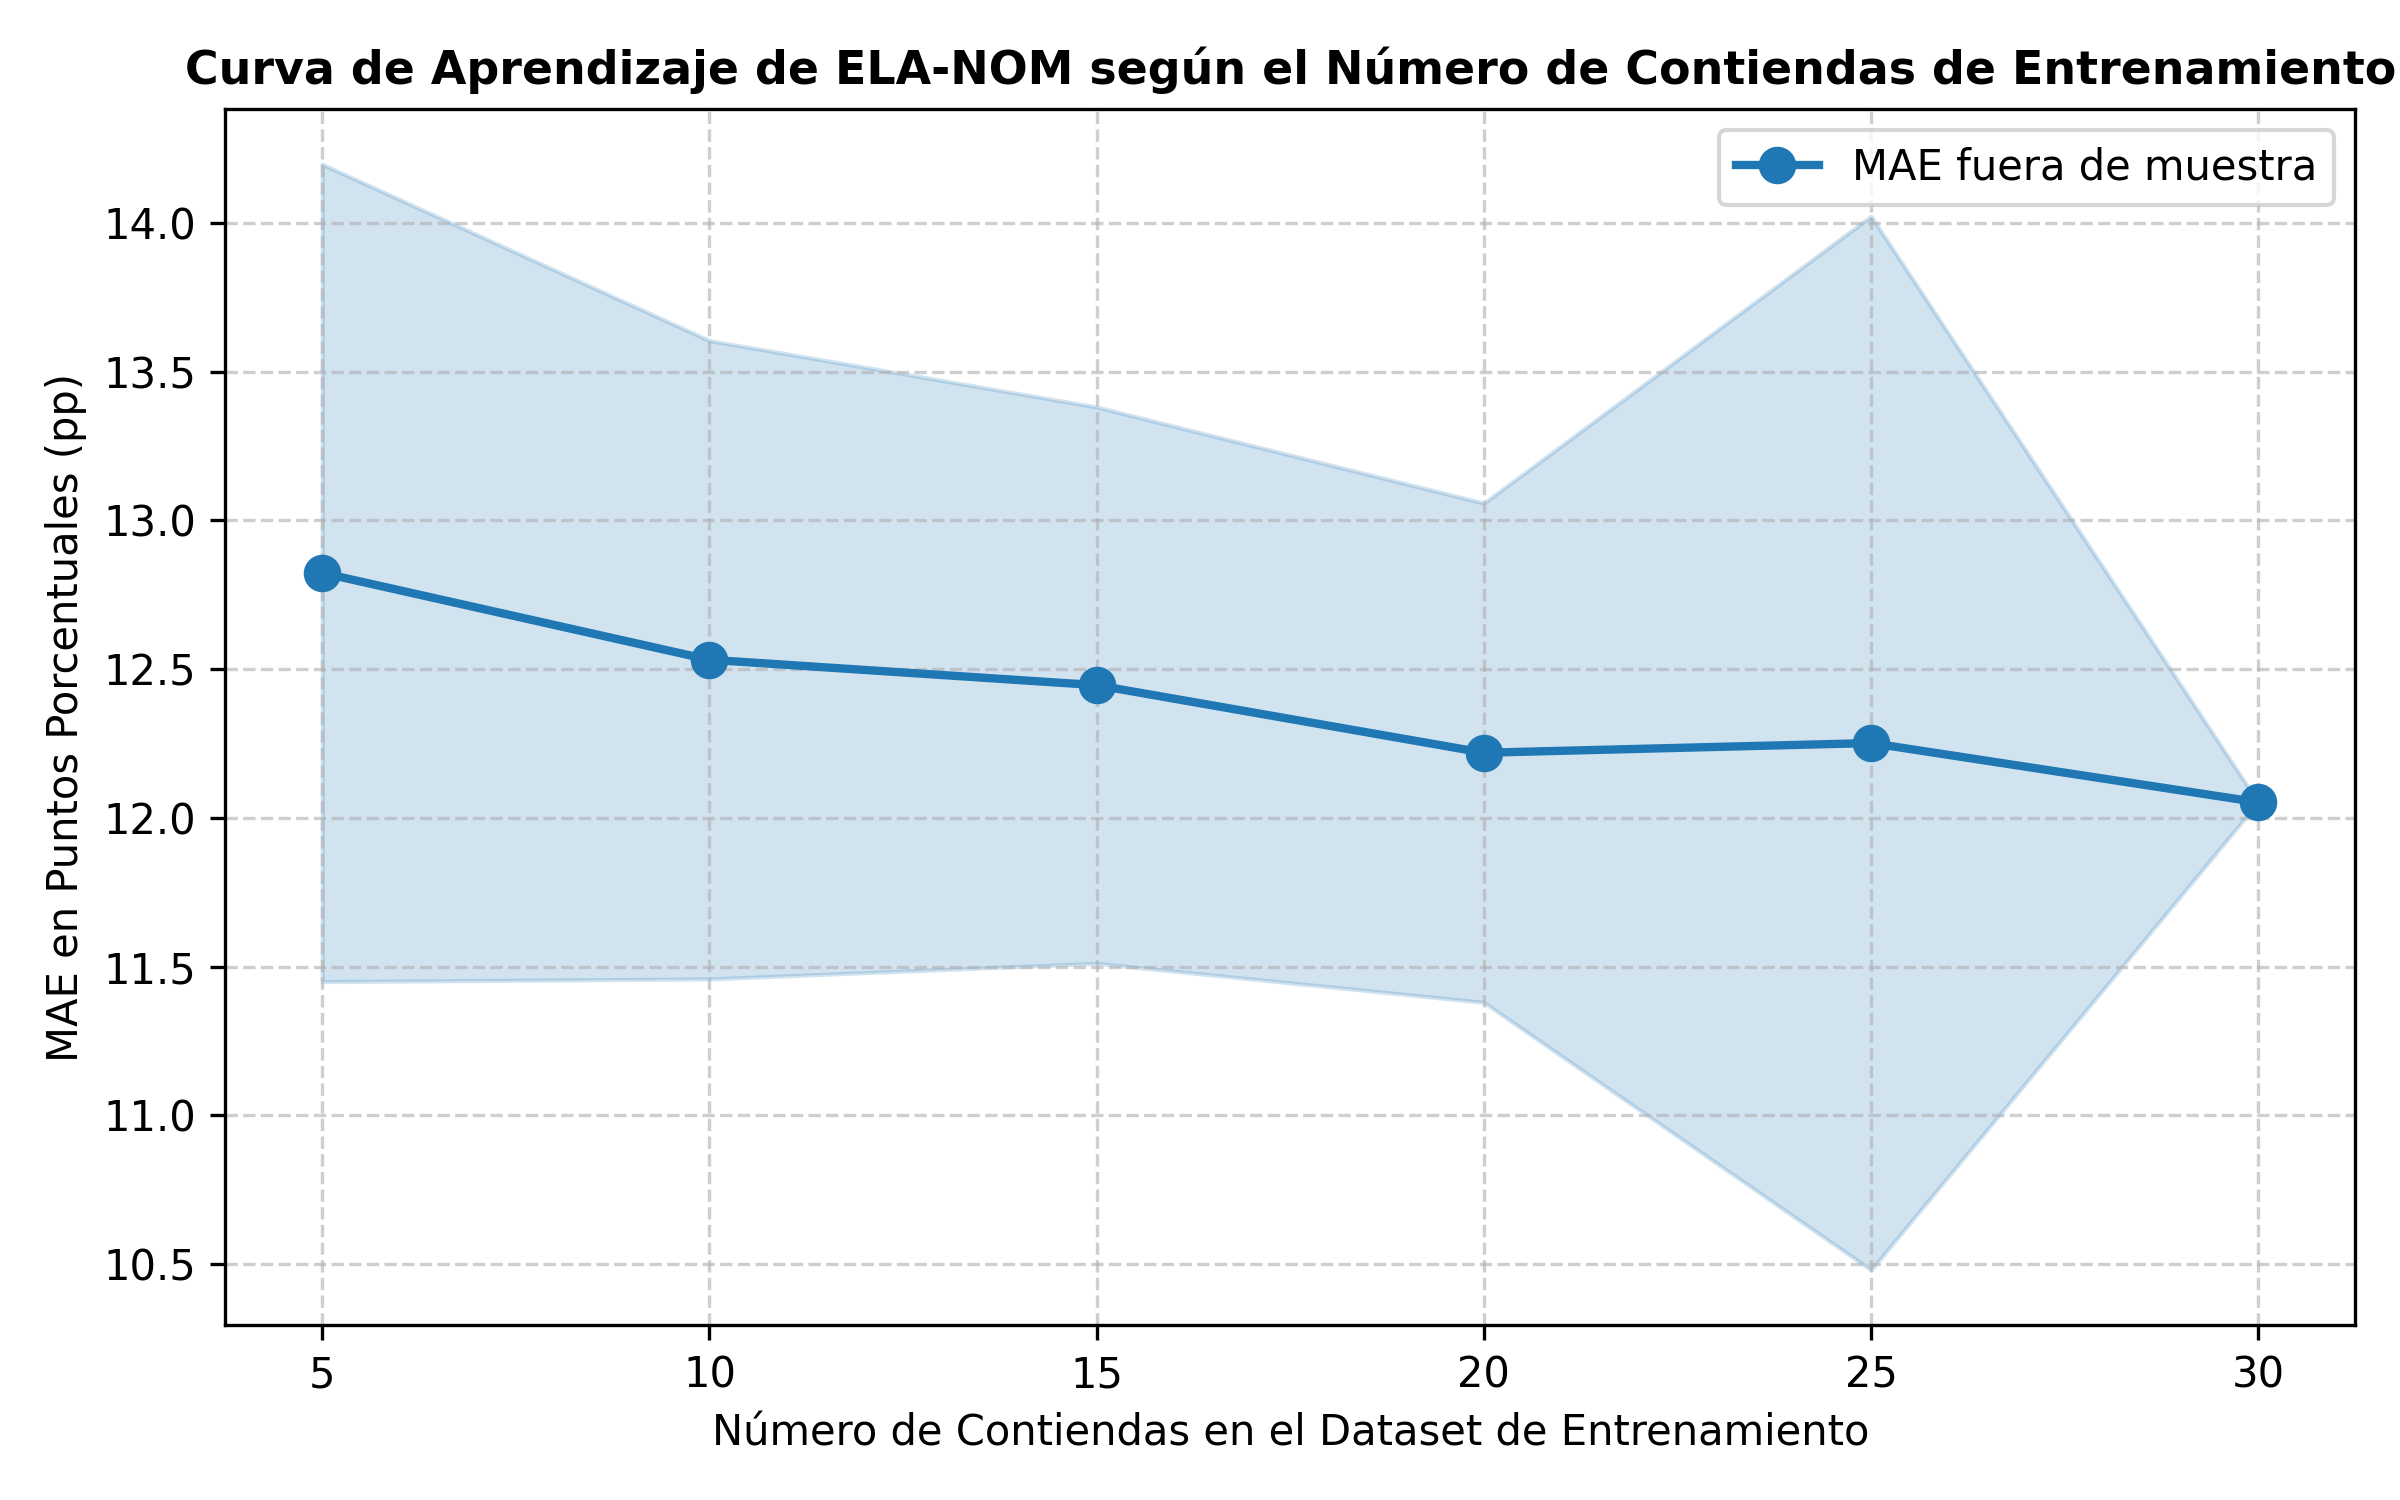
\includegraphics[width=\textwidth]{img/col_learning_curve.png}
    \end{column}
  \end{columns}
\end{frame}

% DIAPOSITIVA 23 (renumerada): Validación 2026 -- datos
\begin{frame}{Validación prospectiva: 2.ª vuelta presidencial 2026}
  \begin{columns}[T]
    \begin{column}{0.52\textwidth}
      \textbf{Cepeda Castro vs.\ De la Espriella}, 21 jun.\ 2026

      \vspace{0.2em}
      \begin{center}\small
      \rowcolors{2}{tableBand}{white}
      \begin{tabular}{L{2.6cm} R{2.2cm} C{1.6cm}}
        \toprule
        \rowcolor{barBlue}
        {\color{white}\textbf{Candidato}} &
        {\color{white}\textbf{Total \textit{likes}}} &
        {\color{white}\textbf{Dom.}} \\
        \midrule
        Cepeda Castro   & 17.087.679 & \num{77,6\%} \\
        De la Espriella &  4.926.361 & \num{22,4\%} \\
        \bottomrule
      \end{tabular}
      \end{center}
      \vspace{0.2em}
      \textbf{Corrección metodológica:}\\
      {\small Modelo entrenado: base aprox.\ 26\% (3,84 candidatos prom.)\\
      2.ª vuelta: base = 50\%; se elimina intercepto:}
      \[
        \hat{p}_c^{(2)} = 0{,}50 + \hat\beta_1 \cdot f_\ell(c)
      \]
      \textbf{Pronósticos:}
      $\hat{p}_{\text{Cepeda}} = \num{60{,}5\%}$,
      $\hat{p}_{\text{Espriella}} = \num{39{,}5\%}$

      \vspace{0.2em}
      {\small \textbf{Trazabilidad} \corr{[Corr.\ 1.15]}: 14 días previos, FB+TW+TikTok,
      444 publicaciones, ElasticNet 2v.\ (random\_state=42)}
    \end{column}
    \begin{column}{0.44\textwidth}
      
\includegraphics[width=\textwidth]{img/col_dominancia_2026.png}
      {\footnotesize\color{subtleGray} Dominancia de \textit{likes}, 444 publicaciones}

      \vspace{0.4em}
      \begin{exampleblock}{\textbf{PM4}: Respondida}
        \small El modelo es \textbf{transferible} a un formato electoral diferente:
        elección presidencial bipolar vs.\ alcaldías multicandidate.
      \end{exampleblock}
    \end{column}
  \end{columns}
\end{frame}

% DIAPOSITIVA 24 (renumerada): Resultado 2026 + corrección MAE
\begin{frame}{Resultado real: contextualización del error \corr{[Corr.\ 1.17/2.4]}}
  \begin{columns}[T]
    \begin{column}{0.52\textwidth}
      \textbf{Resultado real (21 jun.\ 2026):}
      \[
        \text{De la Espriella: } 50{,}48\%
        \quad
        \text{Cepeda: } 49{,}52\%
      \]
      Margen real: \alrt{\textbf{0,96 pp}}, empate técnico.

      \vspace{0.2em}
      \[
        \text{MAE}_{2026} = |60{,}5\% - 49{,}52\%| = \num{10{,}98\,\text{pp}}
      \]
      Supera el MAE medio de entrenamiento en $+1{,}42$ pp.

      \vspace{0.2em}
      \begin{alertblock}{Corrección conceptual: $\pm$MAE no es intervalo}
        \small El MAE mide exactitud promedio, no dispersión.
        ``$\hat{p} \pm \text{MAE}$'' \textbf{no tiene cobertura estadística declarada}.
        Un intervalo formal requiere percentiles de los residuos de LOCO-CV
        o supuestos distribucionales explícitos.
      \end{alertblock}
    \end{column}
    \begin{column}{0.44\textwidth}
      \textbf{Límite estructural:}
      \begin{itemize}\small
        \item Cepeda acumuló 3,5 veces más \textit{likes}; señal real y robusta
        \item Ningún modelo de engagement resuelve contiendas menores a 1 pp
        \item Las encuestadoras colombianas tampoco lo lograron
        \item Factores no capturados: movilización territorial, giros de última semana
      \end{itemize}
      \vspace{0.3em}
      \begin{block}{Uso práctico adecuado del modelo}
        \small ELA-NOM es informativo para ordenar tendencias y detectar
        ventajas mayores a 20 pp. \textbf{No} está diseñado para predecir
        empates técnicos.
      \end{block}
      \vspace{0.2em}
      \begin{exampleblock}{\textbf{PM4}: Delimitado}
        \small El fallo es una condición de borde (margen menor a 1 pp),
        no una falsación del modelo.
      \end{exampleblock}
    \end{column}
  \end{columns}
\end{frame}

% DIAPOSITIVA 26 (renumerada): Conclusiones -- respuesta
\begin{frame}{Conclusiones: respuesta a la pregunta de investigación}
  \begin{block}{\textbf{Sí, es posible. Con matices estructurales bien documentados.}}
    \small MAE$_{\text{oos}}$ = \num{9,56} pp \quad $R^2_{\text{oos}}$ = 0,518 \quad Top-1 = 64,5\% \quad Mejora de \num{3,05} pp sobre baseline \quad Costo: 20--30 USD/ejercicio
  \end{block}

  \vspace{0.2em}
  \begin{columns}[T]
    \begin{column}{0.50\textwidth}
      {\small\textbf{Preguntas respondidas:}}
      \begin{itemize}\scriptsize
        \item \textbf{PM1:} Replicación SOMEN-DC posible. MLP-BP+PCA supera 6$\times$ al baseline
        \item \textbf{PM2:} Las tres limitaciones estructurales confirmadas empíricamente
        \item \textbf{PM3:} Restaurador Weibull -- MAPE Día 3 menor al 13\% en las 4 plataformas
        \item \textbf{P1:} $\rho = 0{,}70$, $p = 0{,}0481$ -- señal predictiva validada
        \item \textbf{P2:} Reconstrucción histórica precisa con parámetros por plataforma
        \item \textbf{P3:} Logit(dominancia \textit{likes}), predictor más robusto y parsimonioso
        \item \textbf{P4:} Con 10 ciudades se alcanza el 95\% del rendimiento final
        \item \textbf{PM4:} Transferible a elección presidencial bipolar sin reentrenamiento
      \end{itemize}
    \end{column}
    \begin{column}{0.46\textwidth}
      {\small\textbf{Limitaciones estructurales:}}
      \begin{itemize}\scriptsize
        \item MAE 9,56 pp: adecuado para tendencias y ventajas mayores a 20 pp; no para empates técnicos
        \item Weibull calibrado en una sola elección (Costa Rica 2026)
        \item Filtro de 10k votos: sesgo de selección sobre v.\ dependiente
        \item Instagram excluida por restricción de API desde 2023
        \item Proxy digital mezcla apoyo, visibilidad, polarización y pauta paga \corr{[2.1]}
      \end{itemize}
    \end{column}
  \end{columns}
\end{frame}

% DIAPOSITIVA 27 (renumerada): Cuatro contribuciones
\begin{frame}{Cuatro contribuciones al estado del arte}
  \begin{enumerate}
    \item \textbf{Elección-agnosticismo empírico}\\
          Primera ruta metodológica demostrada para superar la no-transferibilidad
          del SOMEN-DC: entrenamiento multi-contienda y exportación del núcleo
          a formatos electorales distintos.

    \vspace{0.4em}
    \item \textbf{Independencia demoscópica total}\\
          Único modelo de esta familia que ancla la optimización directamente
          sobre el escrutinio final (el único \textit{ground truth} universal)
          sin depender de encuestas como variable objetivo.

    \vspace{0.4em}
    \item \textbf{Restaurador temporal de series (Weibull)}\\
          Arquitectura matemática para poblar datasets históricos desde una
          extracción estática actual.
          $F(t) = 1 - e^{-k(t+t_0)^{\alpha}}$, parámetros calibrados por plataforma.

    \vspace{0.4em}
    \item \textbf{Democratización del pipeline analítico}\\
          Todo el ciclo (scraping, restauración, modelado con regularización)
          es ejecutable por \textbf{20--30 USD}, varios órdenes de magnitud
          por debajo de una encuesta tradicional.
  \end{enumerate}
\end{frame}

% DIAPOSITIVA 28 (renumerada): Próximos pasos
\addtocounter{framenumber}{1}

% DIAPOSITIVA 29 (renumerada): Cumplimiento de objetivos
\addtocounter{framenumber}{1}

% DIAPOSITIVA 30 (renumerada): Cierre
{
\setbeamertemplate{footline}{}
\begin{frame}[plain]
  \vspace{2.0cm}
  \begin{center}
    {\color{barBlue}\Large\bfseries Gracias}\\[0.5em]
    {\color{barBlue}\rule{0.6\textwidth}{1pt}}\\[0.7em]
    {\color{darkText}\normalsize Juan Sotelo Aguilar}\\[0.2em]
    {\color{subtleGray}\small Maestría en Analítica Aplicada}\\[0.15em]
    {\color{subtleGray}\small Universidad de La Sabana}
  \end{center}
\end{frame}
}


\end{document}
